\documentclass[oneside]{article}
\usepackage[utf8]{inputenc}
\usepackage[dvips]{graphicx}
\usepackage{amsmath}
\title{Anillo Resonante Con Un Punto de Scattering}
\author{Guillem B.G.}
\setlength{\oddsidemargin}{0pt}
\setlength{\evensidemargin}{0pt}

\begin{document}
\maketitle
\newpage
\section{Introducción}
Se busca encontar una fórmula analítica para describir un anillo resonante al
que se le ha introducido un punto de scattering. Como se verá, la posición de
este último no tiene ningún efecto ni sobre la fase, ni sobre la amplitud de la
luz a la salida.

Cuando se simula un sistema como el anterior, se observa que con una elección
adecuada de parámetros, los picos de la resonancia bajan hasta 0 y se desdoblan
por el efecto del acoplamiento entre la luz que gira por el anillo en sentidos
horario y anti-horario en el punto de scattering. Este fenómeno ocurra para
reflectividades en el punto de acoplo tan bajas como el 1\%

\section{Desarrollo}
\subsection{Luz Transmitida}
\begin{figure}[!h]
    \centering
    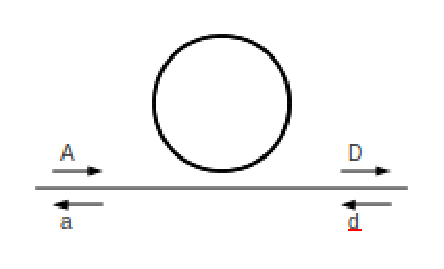
\includegraphics{anillo.eps}
    \caption{Anillo resonante.}
\end{figure}

El siguiente conjunto de matrices describen el acoplamiento entre la guía y los
modos propagantes y contrapropantes en el anillo.

\begin{equation*}
   \begin{pmatrix}
   D \\
   B 
   \end{pmatrix}
   =
   \begin{pmatrix}
      m & ik  \\
      ik & m
   \end{pmatrix}
   \begin{pmatrix}
   A \\
   C 
   \end{pmatrix}
   \qquad
   \begin{pmatrix}
   a \\
   c 
   \end{pmatrix}
   =
   \begin{pmatrix}
      m & ik  \\
      ik & m
   \end{pmatrix}
   \begin{pmatrix}
   d \\
   b 
   \end{pmatrix}
\end{equation*}

La siguiente es la matriz de scattering, que describe el acoplo que ocurre en
el punto de scattering entre los dos modos del anillo.

\begin{equation*}
   \begin{pmatrix}
   C \\
   b 
   \end{pmatrix}
   =
   \begin{pmatrix}
      S_{11} & S_{12}  \\
      S_{21} & S_{22}
   \end{pmatrix}
   \begin{pmatrix}
   c \\
   B 
   \end{pmatrix}
   \quad
   S_{12}=S_{21}
\end{equation*}

Desarrollando y suponiendo que por el puerto de salida no entra luz, se puede
llegar a la siguiente expresión para la respuesta en la salida.

\begin{equation*}
   D = mA -k^{2}\frac{S_{12}(1-mS_{12}) + mS_{11}S_{12}}{(1-mS_{12})^2 - m^2S_{11}S_{12}}A
\end{equation*}
   
Es fácil deducir la siguiente expresión para la matriz de transferencia:

\begin{equation*}
   T = \frac{1}{t}
   \begin{pmatrix}
      e^{ikL} & -re^{ik\Delta}  \\
      -re^{-ik\Delta} & e^{-ikL}
   \end{pmatrix}
   \quad ,
   L = 2\pi R \quad
   \Delta = z' - z
\end{equation*}

donde $t$ y $r$ son la raiz cuadrada de la transmitividad y la reflectividad
cumpliéndose que $t^2 + r^2 = 1$.
La matriz de scattering que le corresponde a $T$ es:

\begin{equation*}
   S =
   \begin{pmatrix}
      -re^{ik(\Delta + L)} & te^{ikL} \\
      te^{ikL} & re^{-ik(\Delta - L)}
   \end{pmatrix}
\end{equation*}

Sustituyendo los parámetros de la matriz $S$ en la ecuación para $D$ y haciendo
el módulo cuadrado llegamos al resultado final

\begin{equation*}
   D^2=\frac{4m^2cos^2(kL)-4mt(m^2+1)cos(kL)+t^2(m^2+1)^2}{4m^2cos^2(kL)-4mt(m^2+1)cos(kL) + (m^2-1)^2 + 4m^2t^2}
\end{equation*}

En la grafica~\ref{picos} se muestran algunos resultados obtenidos a partir de
la expresión anterior.

\subsection{Distancia entre picos}
Como se puede ver en la gráfica~\ref{picos}, a partir de cierta reflectividad 
los picos bajan hasta $0$ y se empiezan a desdoblar. El objetivo de esta sección
es deducir una expresión para evaluar la separación entre los dos picos que
aparecen.

Si se hace cero el numerador de $D^2$ y hacemos el cambio de variable
$y=cos(KL)$ obtenemos la expresión de segundo grado siguiente:

\begin{equation*}
   4m^2y^2 - 4mt(m^2+1)y + t^2(m^2+1)^2 = 0
\end{equation*}

A partir de ella obtenemos el siguiente valor:
\begin{equation*}
   \Delta k_0 = \frac{2}{Ln_{eff}} cos^{-1}\left(\frac{t(m^2+1)}{2m}\right)
\end{equation*}

Adicionalmente imponiendo la condición de que el argumento del arcocoseno sea 
menos que 1, podemos encontrar los valores entre los que puede variar $m$
resolviendo una ecuación de segundo grado.
\begin{equation*}
m_{\pm}=\frac{1\pm r}{t}
\end{equation*}
También habrá que tener en cuenta que $m$ está acotado entre 0 y 1. Lo cual
acaba limitando los posibles valores de $m$ a $[1-r/t,1]$. Esto se puede ver
en la gráfica~\ref{deltak_m}.

Si hubiésemos considerado que la variable erá $t$ habríamos
llegado a la desigualdad:

\begin{equation*}
t < \frac{2m}{m^2+1}
\end{equation*}

\section{Resultados}

En la gráfica~\ref{picos} vemos la luz transmitida en una resonancia para
distintas $R$. Si representásemos más resonancias veríamos que cada vez está
unas más cerca de otras, pero sólo es una consecuencia de haber hecho la gráfica
en función de $\lambda$ en lugar de $k$.
\begin{figure}[h]
    \centering
    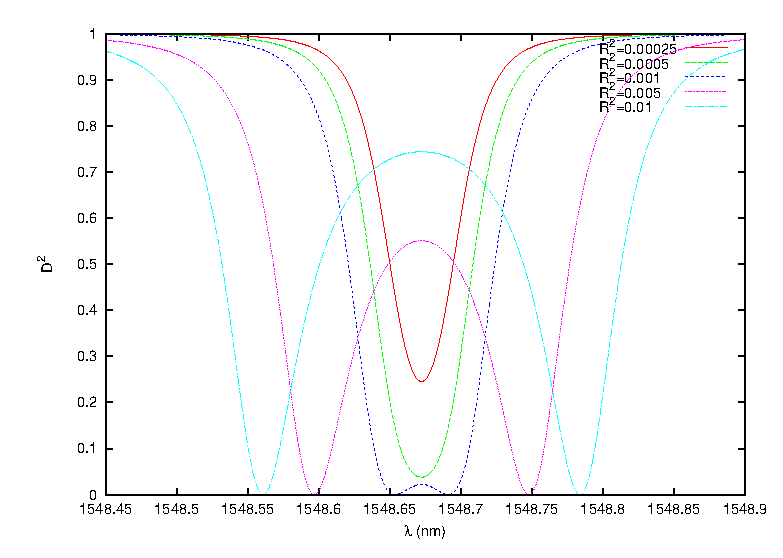
\includegraphics{picos.eps}
    \caption{Ejemplo de una resonancia para distintas $R$. $k^2=0.053$}
    \label{picos}
\end{figure}

En la figura~\ref{deltak_m} observamos como varía $\Delta k$ en función de $m$.
Por debajo del valor $\frac{1- r}{t}$ los picos no llegan hasta 0 y no se
desdoblan. Justo en ese valor se obtiene un único pico ancho que llega a 0.

\begin{figure}[h]
    \centering
    \includegraphics{arcoseno.eps}
    \caption{Distancia entre los picos. $\Delta k=\Delta k_0 n$}
    \label{deltak_m}
\end{figure}

Si en lugar de considerar que el parámetro que varía es $t$ se obtiene la
gráfica~\ref{deltak_t}

\begin{figure}[h]
    \centering
    \includegraphics{deltak_t.eps}
    \caption{Distancia entre los picos. $\Delta k=\Delta k_0 n$ }
    \label{deltak_t}
\end{figure}
\end{document}
